\documentclass{article}

% Encoding
\usepackage[utf8]{inputenc}
% Little tweaks for the margins
\usepackage[margin=2.5cm]{geometry}
% Including graphics
\usepackage{graphicx}

\title{LINFO1252 : Système Informatique}
\author{Nathan Tihon}
\date{\today}



\begin{document}

\maketitle
\newpage

\section{Introduction}

Le but de ce projet est d'implémenter et évaluer les performances de plusieurs algorithmes de synchronisations.
L'évaluation de performances s'articule autour de 2 paramètres, le nombre de \textit{thread} (paramètre entier) et le type de primitive de synchronisation utilisées (paramètre catégoriel).
Le nombre de thread sera un entier comprit entre 1 et $2n$ où $n$ est le nombre de coeurs du processeur utilisé.
Les primitives utilisées appartiendront quant à elle à 2 catégories, la première comprendra les mutex et sémaphores POSIX provenant de \texttt{<pthread.h>} et de \texttt{<semaphore.h>} tandis que la seconde incluera les verrous à attente active (spinlock) ainsi que les sémaphores construites sur ces verrous.

Les figures analysées dans ce rapport suivent toutes la même structure. Elles sont composées de 2 courbes représentant le temps moyen en fonction du nombre de threads, accompagnées de "barres d'erreur" représentant l'écart-type des mesures.
Les couleurs représentent la catégorie de primitives utilisées (paramètre catégoriel), l'axe des abscisses montre le nombre de thread (paramètre entier) et l'axe des orconnées représente le temps d'exécution en fonction de ces paramètres.

Il est à noter que ces figure présentent toutes une valeur nulle pour un thread unique. Cela est dû au fait que nous analysons des algorithmes de \textit{synchronisation}.
Il nous faut donc au minimum 2 threads pour pouvoir analyser le comportement de ces algorithmes.

\section{Verrous à attente active}

Commençons tout d'abord par analyser la performance des spinlocks, car nous utiliseront ceux-ci dans la suite de nos analyses. Il est ici proposé de comparer
2 algorithmes d'implémentation de spinlocks : l'algorithme \textit{test-and-set}, et l'algorithme \textit{test-and-test-and-set} \footnote{Ces algorithmes sont nommées TAS et TATAS pour la suite de ce rapport}.

La figure ci-dessous représente les performances des verrous à attente active.
\begin{figure}[h!]
    \centering
    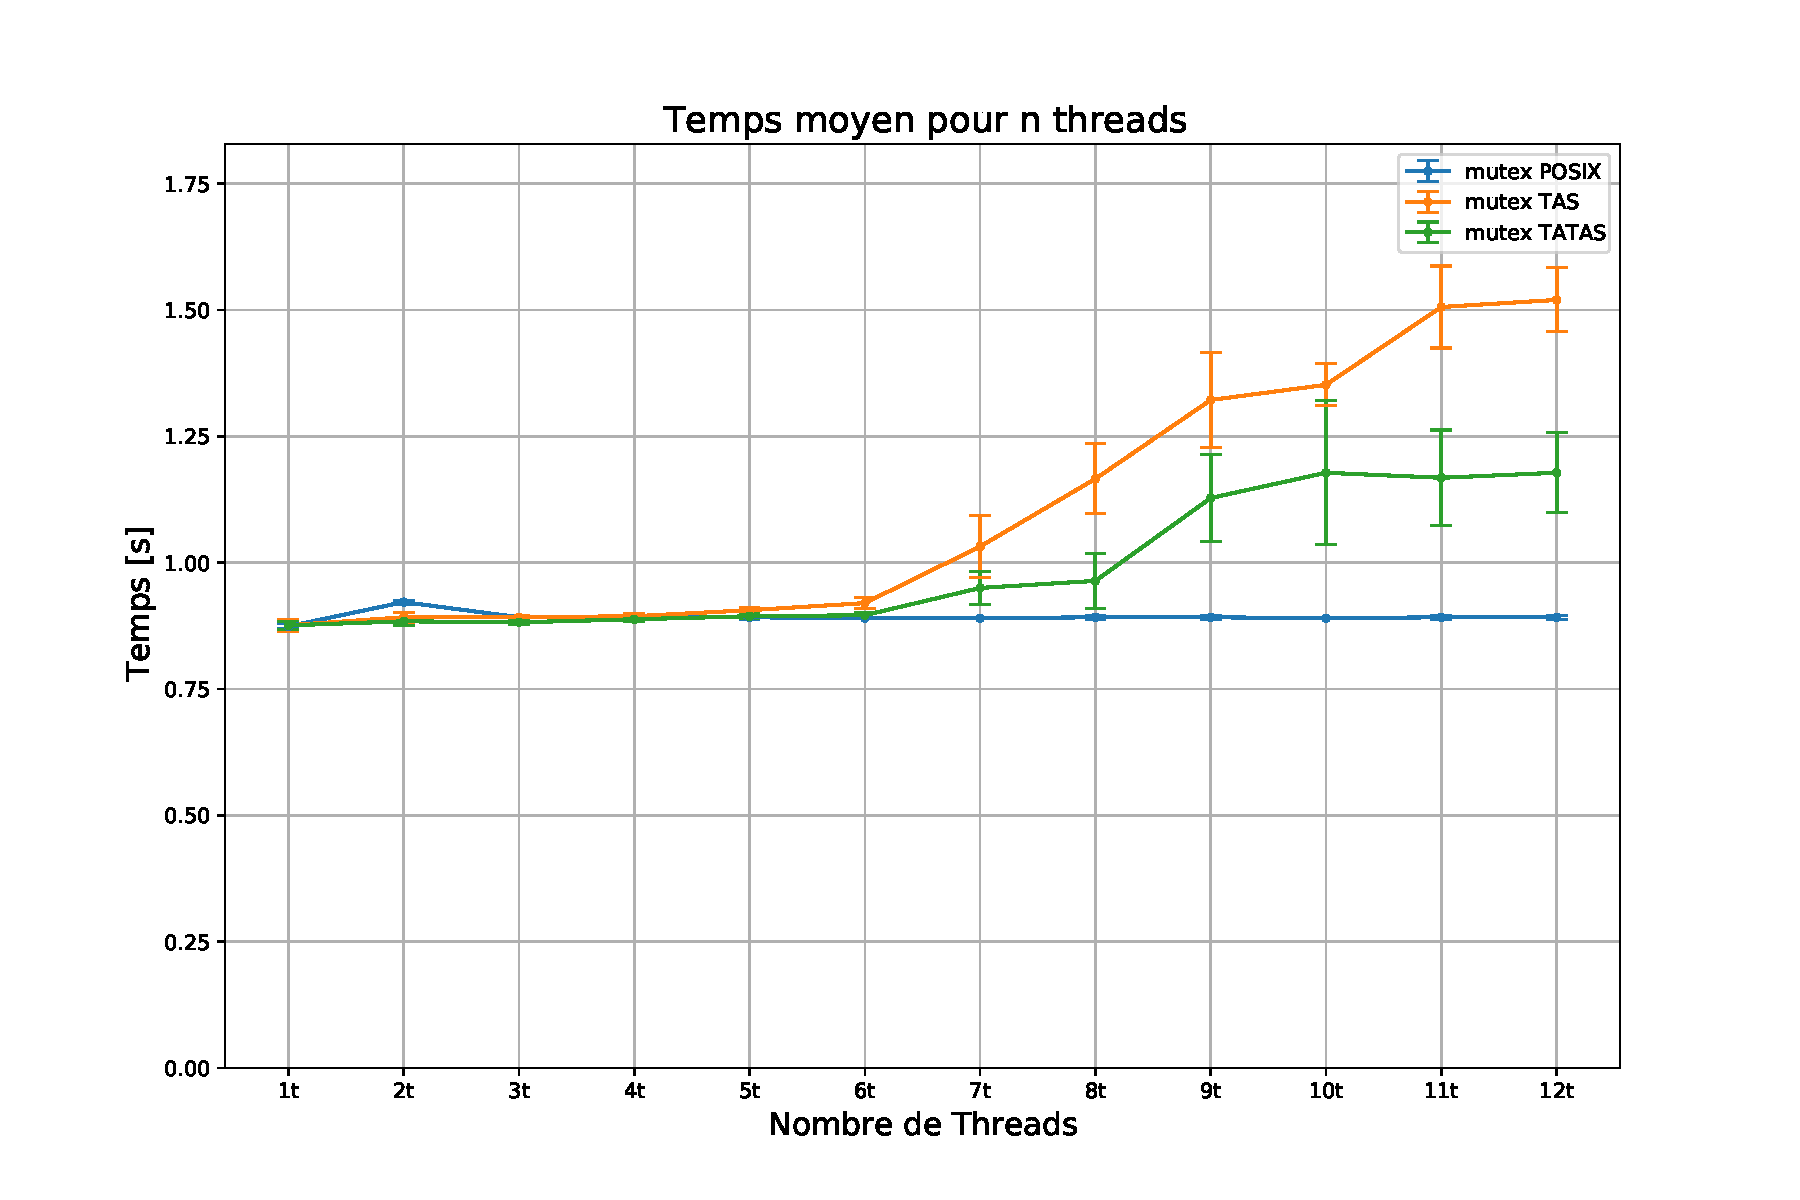
\includegraphics[scale=0.5]{img/spinlock.pdf}
    \caption{Temps d'exécution d'un verrou à attente active dans différentes conditions}
    \label{pic:spinlock}
\end{figure}

Nous pouvons observer que les performances sont assez semblables jusqu'à atteindre un seuil de 6 threads, seuil à partir duquel les performances divergent.
On peut ensuite observer que l'algorithme TATAS performe bien mieux que le TAS, allant parfois jusqu'à un speedup de 20\%. 
Cela peut être expliqué par le fait que l'algorithme TAS, effectue des blocages répétés du bus de cache (à cause de l'instruction \texttt{xchg}) ce qui ralentit considérablement la vitesse à laquelle les différents coeurs synchronisent leur cache (et donc les variables partagées).

\section{Problème des philosophes}

\begin{figure}[h!]
    \centering
    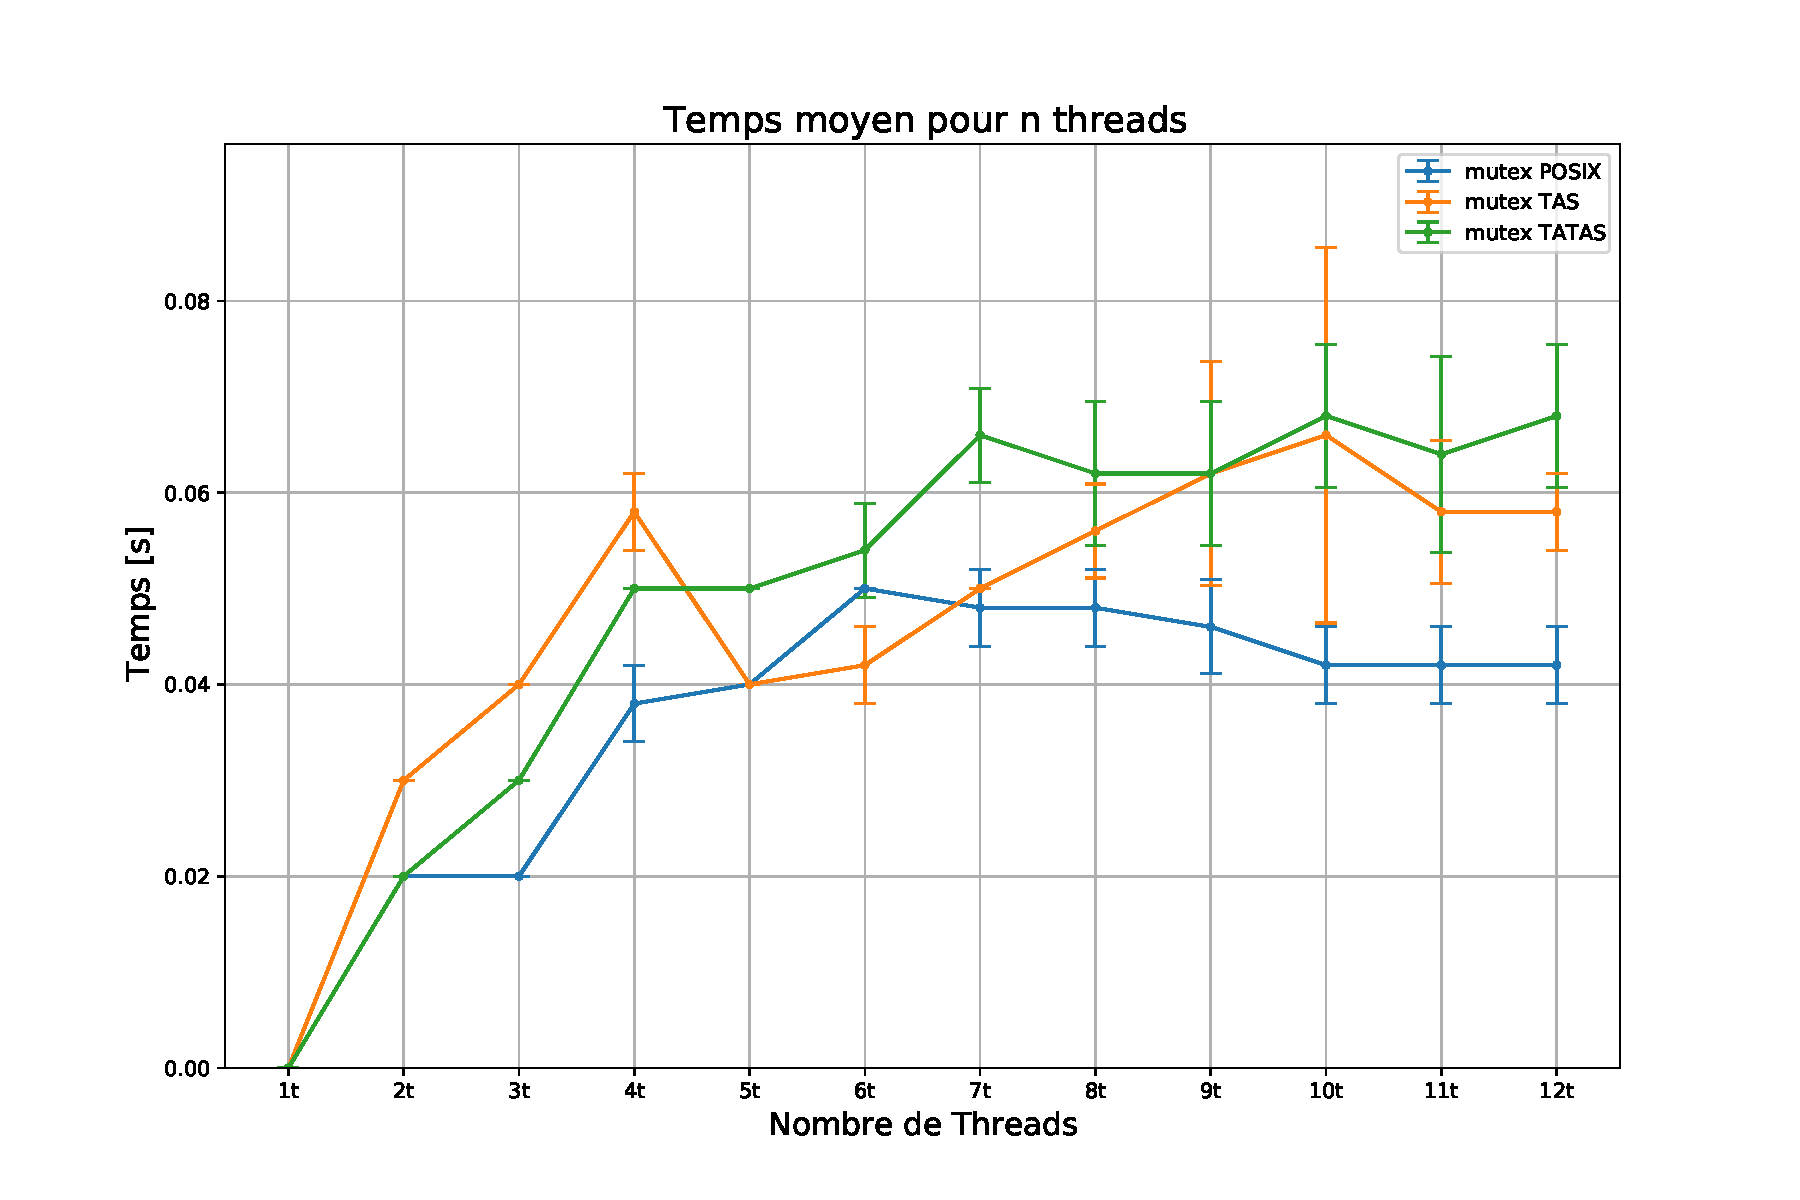
\includegraphics[scale=0.5]{img/philosophes.pdf}
    \caption{Temps d'exécution du problème des philosophes dans différentes conditions}
    \label{pic:philo}
\end{figure}

On remarque que la courbe traitant des mutex POSIX croît jusque 6 threads pour ensuite rester dans la région allant de 0.04 à 0.05 secondes.
Quant à elle, la courbe traitant des spinlock TATAS arrête de croître à 7 threads pour ensuite rester dans la région allant de 0.06 à 0.07 secondes.
On observe également que les mutex POSIX sont généralement plus stable que les spinlock TATAS. En effet on voit clairement que l'écart-type est bien inférieur.

L'allure générale des deux courbes peut être expliquée par le simple fait qu'ajouter des threads revient à ajouter du travail.
Ces deux observations (meilleur temps d'exécution et stabilité) peuvent être expliquées par le fait que ...


\section{Problème des Producteurs-Consommateurs}

\begin{figure}[h!]
    \centering
    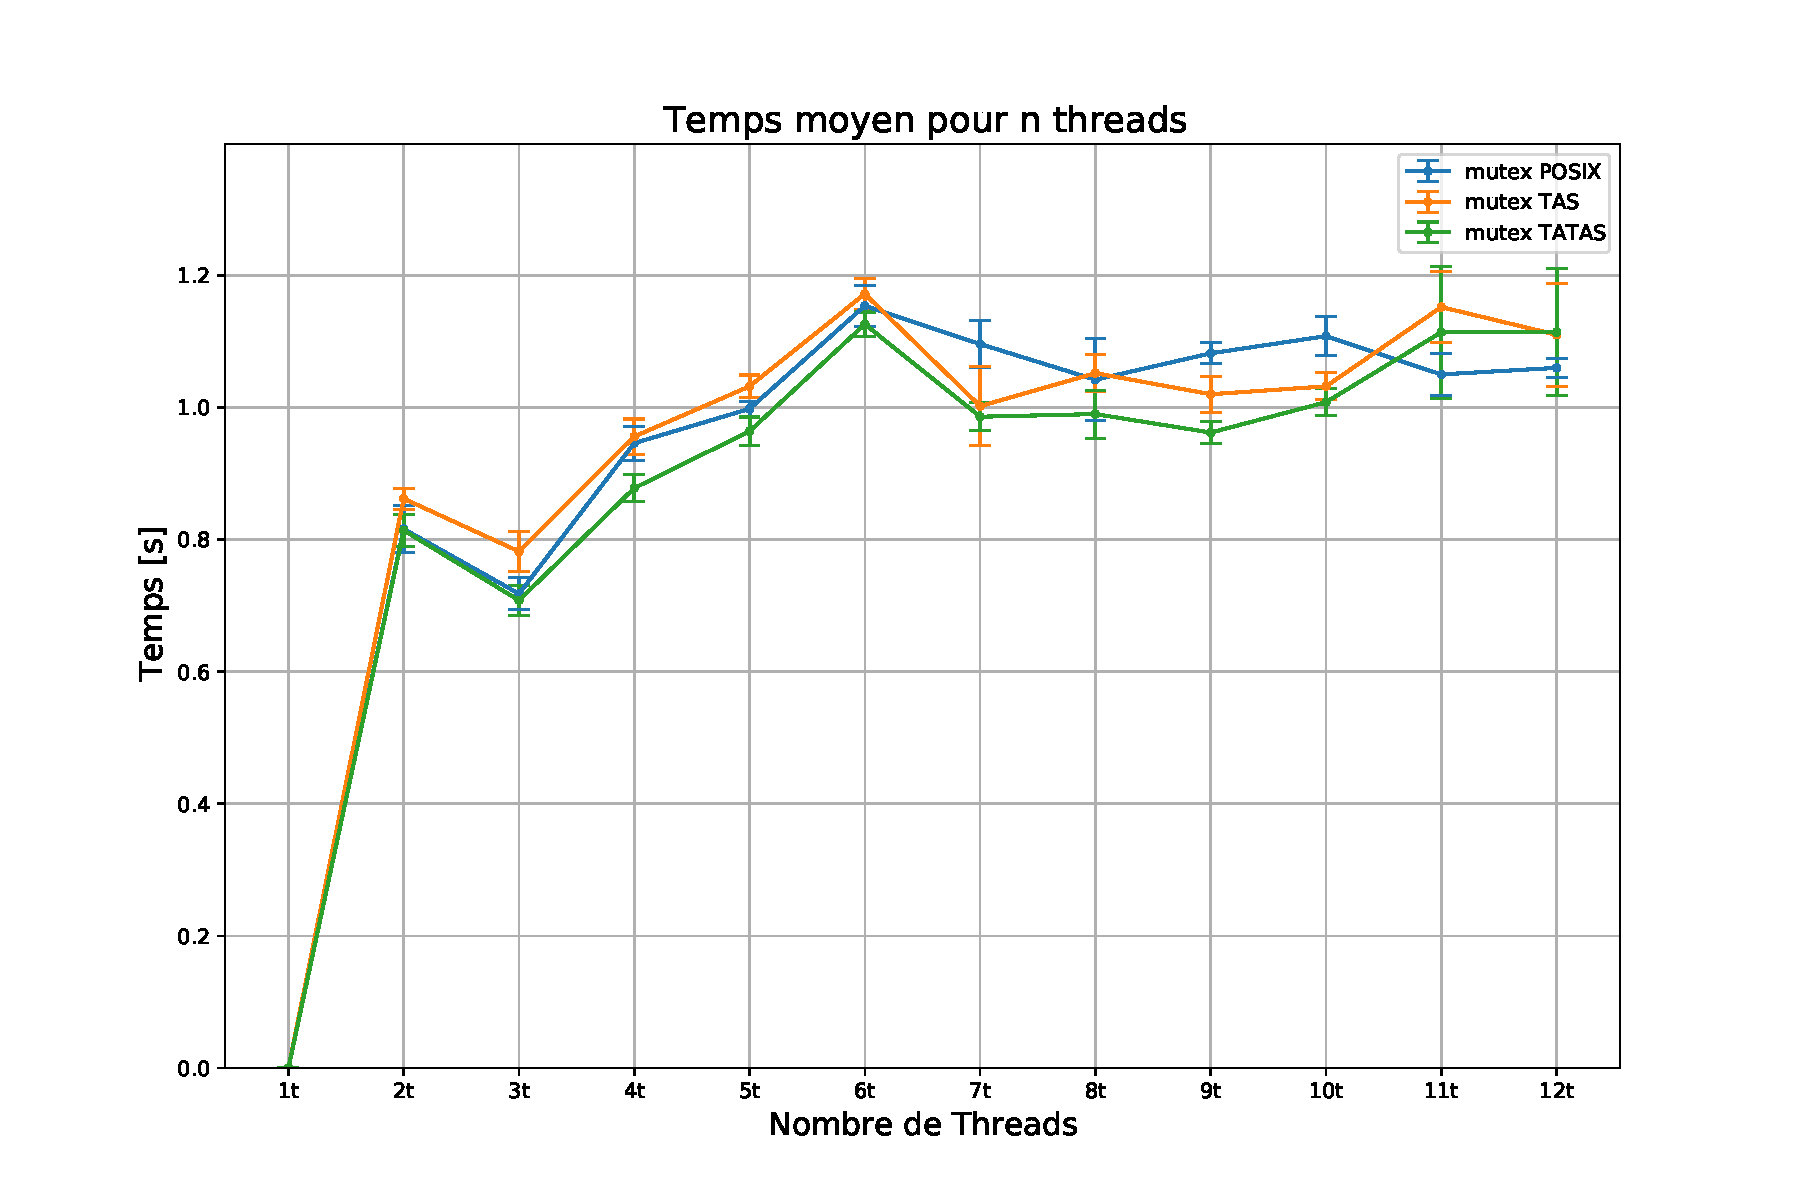
\includegraphics[scale=0.5]{img/prodcons.pdf}
    \caption{Temps d'exécution du problème des producteurs-consommateurs dans différentes conditions}
    \label{pic:prodcons}
\end{figure}

Remarquons premièrement que le comportement des deux courbes de 2 à 10 threads est très similaire pour ensuite aboutir à un croisement des deux courbes entre 10 et 11 threads.
On remarque une diminution de 2 à 3 threads pour ensuite avoir une augmentation jusqu'à 6 threads et une stabilisation.


\section{Problème des lecteurs-écrivains}



\begin{figure}[h!]
    \centering
    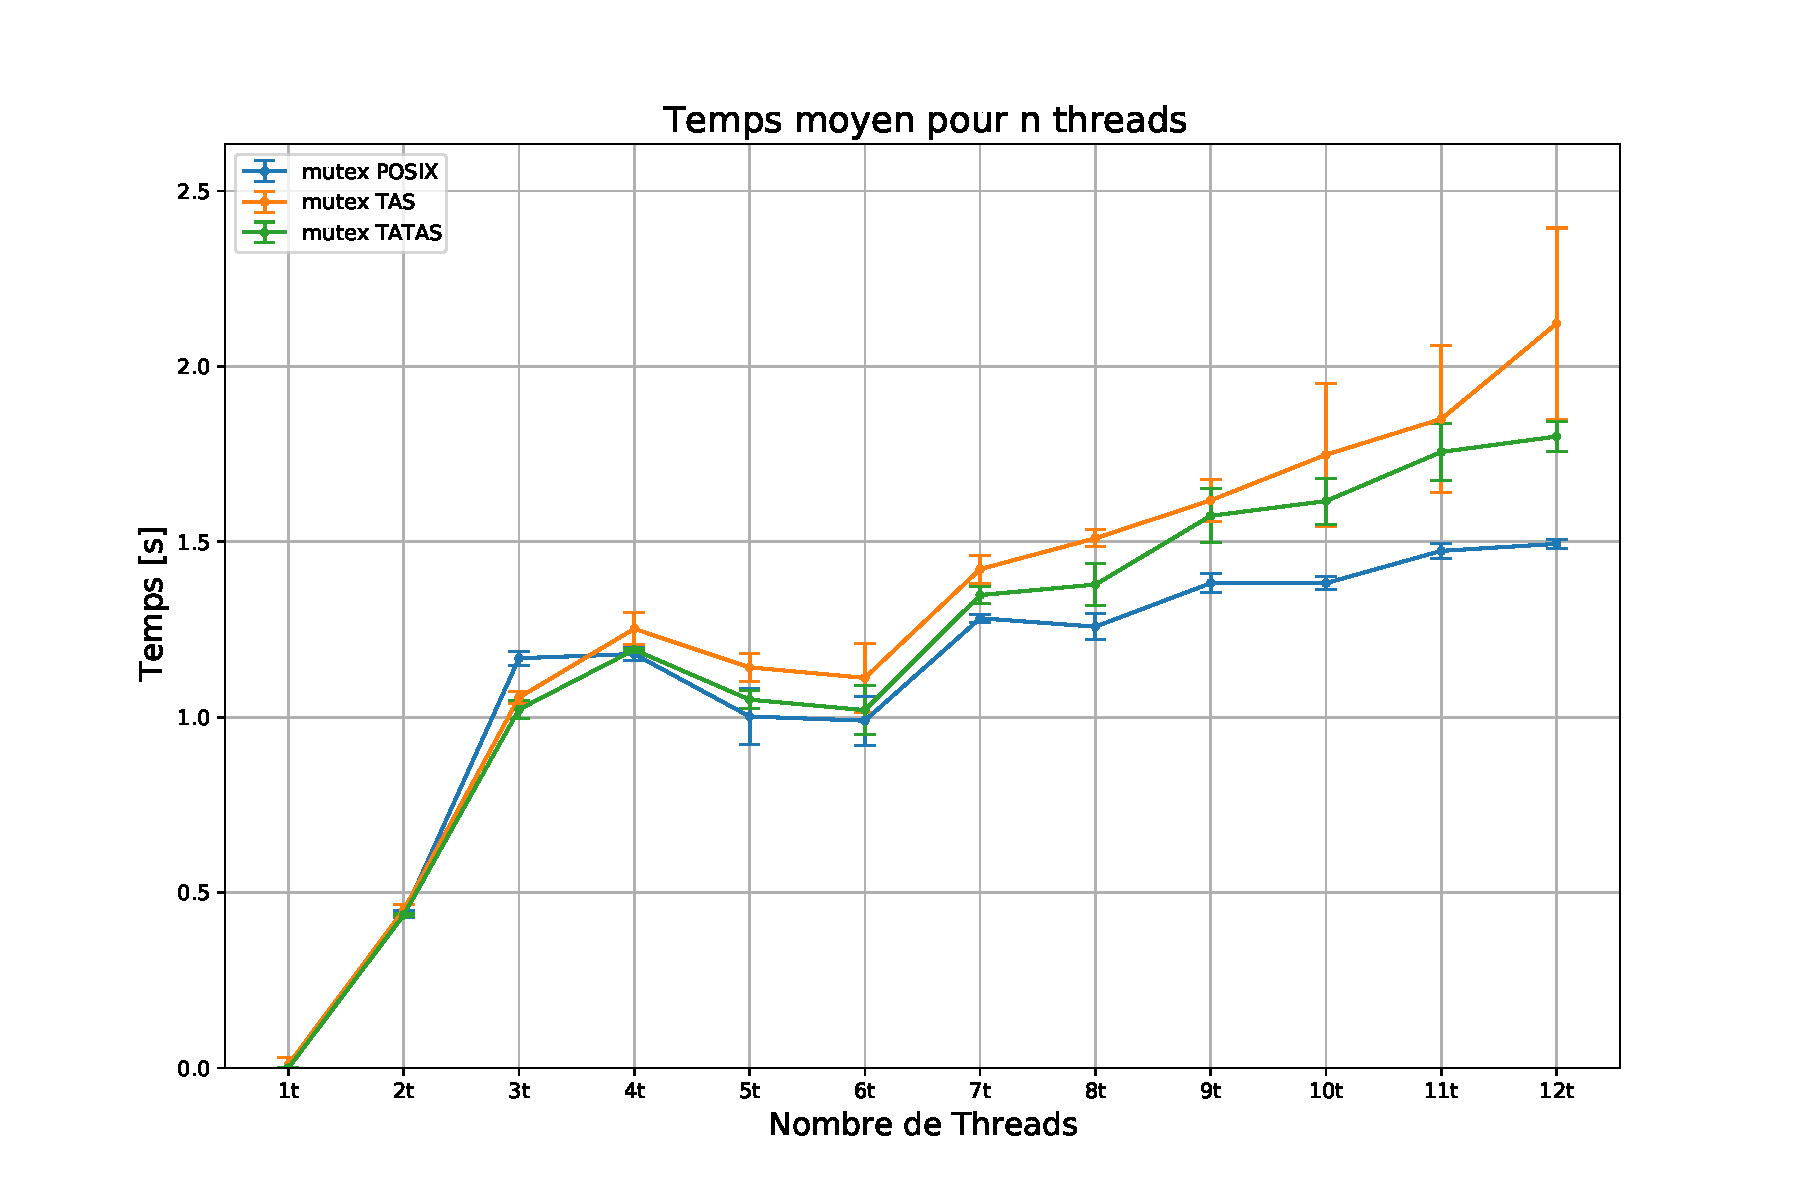
\includegraphics[scale=0.5]{img/readwrt.pdf}
    \caption{Temps d'exécution du problème des lecteurs-écrivains dans différentes conditions}
    \label{pic:readwrt}
\end{figure}

\end{document}

\section{Conclusion}